%%%%%%%%%%%%%%%%%%%%%%%%%%%%%%%%%%%%%%%%%
% Stylish Article
% LaTeX Template
% Version 2.0 (13/4/14)
%
% This template has been downloaded from:
% http://www.LaTeXTemplates.com
%
% Original author:
% Mathias Legrand (legrand.mathias@gmail.com)
%
% License:
% CC BY-NC-SA 3.0 (http://creativecommons.org/licenses/by-nc-sa/3.0/)
%
%%%%%%%%%%%%%%%%%%%%%%%%%%%%%%%%%%%%%%%%%

%----------------------------------------------------------------------------------------
%	PACKAGES AND OTHER DOCUMENT CONFIGURATIONS
%----------------------------------------------------------------------------------------

\documentclass[fleqn,10pt]{SelfArx} % Document font size and equations flushed left

\usepackage{lipsum} % Required to insert dummy text. To be removed otherwise


%----------------------------------------------------------------------------------------
%	Source Code Listings
%----------------------------------------------------------------------------------------
\usepackage{listings}
\usepackage{xcolor}
\definecolor{darkgreen}{rgb}{0.0, 0.2, 0.13}
\definecolor{ao}{rgb}{0.0, 0.5, 0.0}
\lstdefinestyle{sharpc}{language=[Sharp]C, frame=single}
\lstset{% general command to set parameter(s)
basicstyle=\small, % print whole listing small
keywordstyle=\color{blue}\bfseries,
% underlined bold black keywords
commentstyle=\small\color{ao}, % white comments
stringstyle=\ttfamily, % typewriter type for strings
columns=fullflexible, % keeps the comments from exploding
showstringspaces=false} % no special string spaces


%----------------------------------------------------------------------------------------
%	COLUMNS
%----------------------------------------------------------------------------------------

\setlength{\columnsep}{0.55cm} % Distance between the two columns of text
\setlength{\fboxrule}{0.75pt} % Width of the border around the abstract

%----------------------------------------------------------------------------------------
%	COLORS
%----------------------------------------------------------------------------------------

\definecolor{color1}{RGB}{0,0,90} % Color of the article title and sections
\definecolor{color2}{RGB}{0,20,20} % Color of the boxes behind the abstract and headings

%----------------------------------------------------------------------------------------
%	HYPERLINKS
%----------------------------------------------------------------------------------------

\usepackage{hyperref} % Required for hyperlinks
\hypersetup{hidelinks,colorlinks,breaklinks=true,urlcolor=color2,citecolor=color1,linkcolor=color1,bookmarksopen=false,pdftitle={Title},pdfauthor={Author}}

%----------------------------------------------------------------------------------------
%	ARTICLE INFORMATION
%----------------------------------------------------------------------------------------

\JournalInfo{PBIP \#78, 2015} % Journal information
\Archive{Additional note} % Additional notes (e.g. copyright, DOI, review/research article)

\PaperTitle{PacBio Improvement Proposal \#((int)`N`) \\{\large Removing the deletion tag value from secondary analysis}} % Article title

\Authors{Nigel Delaney} % Authors

\Keywords{} % Keywords - if you don't want any simply remove all the text between the curly brackets
\newcommand{\keywordname}{Keywords} % Defines the keywords heading name

%----------------------------------------------------------------------------------------
%	ABSTRACT
%----------------------------------------------------------------------------------------

\Abstract{ The PacBio consensus calling framework is greatly complicated by the presence of deletion tag values attached to certain basepairs.  These  that are emitted by the .}

%----------------------------------------------------------------------------------------

\begin{document}

\flushbottom % Makes all text pages the same height

\maketitle % Print the title and abstract box

\tableofcontents % Print the contents section

\thispagestyle{empty} % Removes page numbering from the first page

%----------------------------------------------------------------------------------------
%	ARTICLE CONTENTS
%----------------------------------------------------------------------------------------

\section*{Introduction} % The \section*{} command stops section numbering

\addcontentsline{toc}{section}{Introduction} % Adds this section to the table of contents

A desirable statistical model is no more complex than necessary, does not contain unnecessary parameters and has a likelihood function that is smooth and continuous to aid in optimization.  There should also be a well defined generative process that defines how the observed data should be interpreted.

The use of Deletion Tags (DelTags), in secondary analysis takes the CCS and Quiver models further away from, rather than closer to, this ideal.  The proposal suggests that either DelTag values should be removed entirely, or the deleted base should be promoted to an actual base in the read sequence, so that it could be handled using the framework for insertions/deletions present in the scoring models that does not require DelTags. 

Here, I review the origin and rational for deletions tags then present several arguments for their removal. 



\subsection{What are DelTags?}
Each base in a PacBio dataset may have an associated DelTag value which is one of the basepairs A, C, G, T.  It is defined in the PacBio documentation as the \textit{``Likely identity of a deleted base, if it exists"}.  In practice, typically approximately 10\% of bases in a dataset will have this value, the remainder will have an 'N' value. The DeletionTag value is created within the method that converts pulses into bases\footnote{Method: \texttt{ AnalyzeInsertClassify@PulseToBaseStream.cs:521}}.

Before discussing when and how DelTags are added, it is worth mentioning that generally speaking, the Deletion QV values emitted from Primary are not very useful, and their calculation appears to be an unfinished project in primary analysis.  It appears Pat originally intended to create Deletion QV values using a GBM to predict the likelihood of error, as is currently done for insertion QVs.  However, at present the values for the deletion QV are all hardcoded to a QV of 17 with the following line of code:\footnote{\texttt{PulseToBaseStream.cs:478}}

\lstset{style=sharpc}
\begin{lstlisting}[frame=single]
/* This could be done much more intelligently.
  We weren't really able to get a DeletionClassifier
  to give much benefit. */
delPrediction = incPredictions.Map(v => 0.02f);
\end{lstlisting}

Although all DeletionQV values are initially hard-coded to the seemingly arbitrary 17 value in PulseToBases, this value can later be modified if and only if when converting Pulses to Bases some pulses are not emitted, or are skipped.  If a pulse is skipped, then a new DeletionQV value, and a DelTag, is attached to the next pulse converted to a base.  This is the only time a DelTag will exist.

To obtain both the base and the QV value, the skipped pulses are all evaluated.  The basepair of the skipped pulse with the highest probability of incorporation becomes the DelTag basepair.  A new DeletionQV value is then calculated as the sum of all the deletion probabilities for the skipped bases (which are all a fixed constant), plus the probability of incorporation for the most likely base.  The specific code to do this is shown below.\footnote{\texttt{PulseToBaseStream.cs:636}}

\lstset{style=sharpc}
\begin{lstlisting}[frame=single]
// sum up all the deletion probability since the last base
float dqvs1 = 0.0;
// We did skip some pulses since the last base
// For now lets just consider the one that was closest to being a base
float skippedIncMax = float.MinValue;
int worstSkippedPulseIndex = 0;
// This could use a bit of attention
foreach(var p in skippedPulses) {
    if(incPredictions[p] > skippedIncMax)    {
        skippedIncMax = incPredictions[p];
        worstSkippedPulseIndex = p;
    }
    dqvs1 += delPredictions[p];
}
/*  Total probability of a deletion is the sum of the bg deletion rates 
over the gaps, plus the incorporation probability of the leftover 
pulse. */
delProb = dqvs1 + incPredictions[worstSkippedPulseIndex];
delQV.Add(QVs.ProbToQV(delProb));
delTag.Add(iBases[worstSkippedPulseIndex]);
\end{lstlisting}

This code appears wrong from a number of perspectives.  First, when considering deletion events before each pulse, this code sums the deletion probabilities before each base which is incorrect. The correct calculation, given the fixed value of 0.02 for $N$ skipped pulses would be to account for the probability that there were no deletions before each pulse as: $ (1 - (1-.02)^N)$.  Fortunately, because the fixed constant currently used is small, the summation used and the correct formula give similar results as $(1-0.02)^N \thickapprox 1 - N\cdot0.02$.  However, this will not generally be true for larger fixed constants and/or a large number of skipped pulses.

The second issue is that only the pulse with the highest probability of being a true incorporation is considered.  The correct formula for multiple skipped pulses would be similar to the one for deletions, but replacing the fixed constant with the value for each pulses incorporation probability.  If there is only one skipped base, these two approaches are equivalent, but if there are multiple skipped pulses, they are again distinct.


 



%------------------------------------------------

\section{Arguments Against DelTags}

\begin{figure*}[ht]\centering % Using \begin{figure*} makes the figure take up the entire width of the page
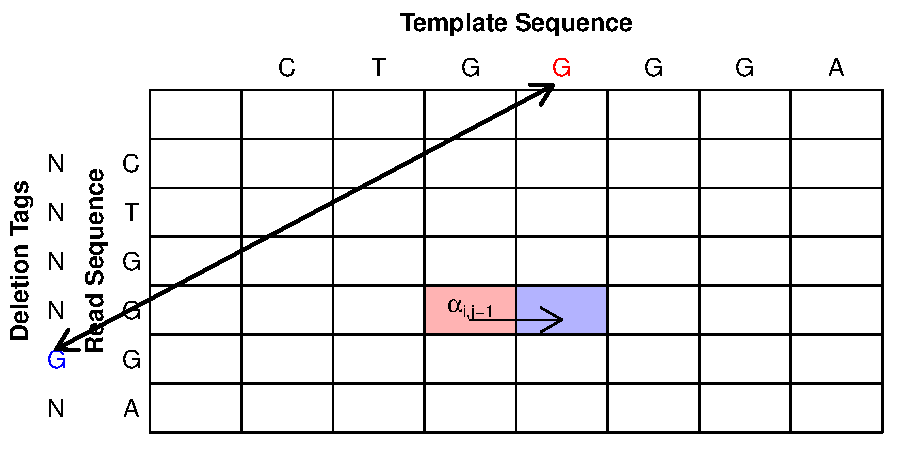
\includegraphics[width=\linewidth]{Deletion}
\caption{Deletion Scoring}
\label{fig:del}
\end{figure*}

\subsection{They make scoring complex}

The "Deletion Move" in our template scoring routine is done in one of two distinct ways depending on if a Deletion Tag is present.  With positions denoted by Figure \ref{fig:del}, a Deletion move is currently scored according to the template shown below.  
\[
	\alpha_{i,j-1}  +  \begin{cases}
							 \text{Deletion score  for } R_{i+1}  & \text{if }  \text{DeletionTag}_{i+1} = T_{j} \\
							 \text{A fixed constant} & \text{if }  \text{DeletionTag}_{i+1} \neq T_{j} 
							 \end{cases}
\]

By having two possible scoring methods, we not only need to estimate 3 parameters for the deletion move in training, but we also are scoring the same behavior (a deletion in the template), using two separate methods.


\lipsum[5] % Dummy text

\begin{enumerate}[noitemsep] % [noitemsep] removes whitespace between the items for a compact look
\item First item in a list
\item Second item in a list
\item Third item in a list
\end{enumerate}

\subsection{Subsection}

\lipsum[6] % Dummy text

\paragraph{Paragraph} \lipsum[7] % Dummy text
\paragraph{Paragraph} \lipsum[8] % Dummy text

\subsection{Subsection}

\lipsum[9] % Dummy text



Reference to Figure \ref{fig:results}.

%------------------------------------------------

\section{Results and Discussion}

\lipsum[10] % Dummy text

\subsection{Subsection}

\lipsum[11] % Dummy text

\begin{table}[hbt]
\caption{Table of Grades}
\centering
\begin{tabular}{llr}
\toprule
\multicolumn{2}{c}{Name} \\
\cmidrule(r){1-2}
First name & Last Name & Grade \\
\midrule
John & Doe & $7.5$ \\
Richard & Miles & $2$ \\
\bottomrule
\end{tabular}
\label{tab:label}
\end{table}

\subsubsection{Subsubsection}

\lipsum[12] % Dummy text

\begin{description}
\item[Word] Definition
\item[Concept] Explanation
\item[Idea] Text
\end{description}

\subsubsection{Subsubsection}

\lipsum[13] % Dummy text

\begin{itemize}[noitemsep] % [noitemsep] removes whitespace between the items for a compact look
\item First item in a list
\item Second item in a list
\item Third item in a list
\end{itemize}

\subsubsection{Subsubsection}

\lipsum[14] % Dummy text

\subsection{Subsection}

\lipsum[15-23] % Dummy text

%------------------------------------------------
\phantomsection
\section*{Acknowledgments} % The \section*{} command stops section numbering

\addcontentsline{toc}{section}{Acknowledgments} % Adds this section to the table of contents

So long and thanks for all the fish \cite{Figueredo:2009dg}.

%----------------------------------------------------------------------------------------
%	REFERENCE LIST
%----------------------------------------------------------------------------------------
\phantomsection
\bibliographystyle{unsrt}
\bibliography{sample}

%----------------------------------------------------------------------------------------

\end{document}